% !TEX TS-program = pdflatexmk
\documentclass[12pt, letterpaper, titlepage]{article}

\makeatletter
\g@addto@macro\@floatboxreset\centering
\makeatother

\usepackage{amsmath}
\usepackage{booktabs}
\usepackage{amsthm}
\usepackage{graphicx}
\usepackage[margin=1in]{geometry}
\usepackage{hyperref}
\hypersetup{colorlinks = true, linkcolor = blue, citecolor=blue, urlcolor = blue}
\usepackage{natbib}
\usepackage{enumitem}
\usepackage{float}
\usepackage{tikz}
\usepackage{setspace}

\usepackage[pagewise]{lineno}
%\linenumbers*[1]
% %% patches to make lineno work better with amsmath
\newcommand*\patchAmsMathEnvironmentForLineno[1]{%
 \expandafter\let\csname old#1\expandafter\endcsname\csname #1\endcsname
 \expandafter\let\csname oldend#1\expandafter\endcsname\csname end#1\endcsname
 \renewenvironment{#1}%
 {\linenomath\csname old#1\endcsname}%
 {\csname oldend#1\endcsname\endlinenomath}}%
\newcommand*\patchBothAmsMathEnvironmentsForLineno[1]{%
 \patchAmsMathEnvironmentForLineno{#1}%
 \patchAmsMathEnvironmentForLineno{#1*}}%

\AtBeginDocument{%
 \patchBothAmsMathEnvironmentsForLineno{equation}%
 \patchBothAmsMathEnvironmentsForLineno{align}%
 \patchBothAmsMathEnvironmentsForLineno{flalign}%
 \patchBothAmsMathEnvironmentsForLineno{alignat}%
 \patchBothAmsMathEnvironmentsForLineno{gather}%
 \patchBothAmsMathEnvironmentsForLineno{multline}%
}

% control floats
\renewcommand\floatpagefraction{.9}
\renewcommand\topfraction{.9}
\renewcommand\bottomfraction{.9}
\renewcommand\textfraction{.1}
\setcounter{totalnumber}{50}
\setcounter{topnumber}{50}
\setcounter{bottomnumber}{50}

\newcommand{\jy}[1]{\textcolor{blue}{JY: #1}}
\newcommand{\eds}[1]{\textcolor{red}{EDS: (#1)}}

%% meta data

\title{Sentiment Analysis of Twitter in Relation to Fossil Fuel Stock Prices}
\author{Pranav Tavildar\\
  University of Connecticut \\
  Advisor: Jun Yan\\
  Department of Statistics\\
  University of Connecticut
}

\begin{document}
\maketitle
\doublespace

\begin{abstract}
As a publicly traded company, the Chevron Corporation has the 11th highest market capitalization in the world with 361.57 billion dollars in traded stocks. There exist many social factors that contribute to this stock value but this paper aims to establish a methodology to test whether twitter sentiment is informative in predicting stock price movement and its volatility for the Chevron Corporation stock(CVX). This is done by using a DistilBert transformer architecture to assign a sentiment score for each tweet and afterwords, we try to determine if there is a correlation between stock price and daily sentiment using an ARMA GARCH Model.


\jy{alphabetical; no repeating words in title. Read my writing tips and practice them}
\bigskip
\noindent{\sc Keywords}:
BERT;
chevron;
twitter;
nlp;
sentiment analysis.

\end{abstract}

\jy{what do I recommend for linewidth?}

\jy{Two figure labels are multiply defined. Read the log and fix the warnings}
%%%%%%%%%%%%%%%%%%%%%%%%%%%%%%%%%%%%%%%%%%%%%%%
\section{Introduction}
\label{sec: intro}
%\paragraph{Overview of topic}

The Chevron Corporation is an America-based energy company thats has operations in over 180 countries where it has vertically integrated all operations in its supply chain such as exploration, production, refinement, chemical manufacturing, transportation, sales, marketing, and power generation. A lot of revenue comes from these streams but they also receive funding from government subsidies and stock revenue. As of when this paper was written, the Chevron Corporation has the 11th highest market capitalization with 361.57 billion dollars in traded stocks.

As a publicly traded company, Chevron's stock price is determined by supply and demand in the market. Generally, this is influenced by factors such as market dynamics, economic conditions and changes to economic policy. Through this paper, we seek to determine whether this can be predicted or determined through observing public speculation on Twitter, the "virtual public square." Being able to determine whether public sentiment can be informative in predicting stock price might prove as a valuable indicator for many groups such as investors, activists, and companies officials to determine how much of a correlation a change in public opinion has to the stock value.  	
%\paragraph{Review of the Literature}

To quantify public opinion, this paper uses a machine learning technique known as sentiment analysis \citep{medhat2014sentiment} which uses natural language processing to determine whether the sentiment towards any subject is positive or negative and assigns it a score.

 Some papers in the literature use this technique in relation to analyzing activity in the stock market. Koosha Golmohammadi and Osmar R. Zaiane for instance use sentiment analysis with Twitter data to improve their Contextual Anomaly Detection(CAD) model in order to detect Market Manipulation in the United States and Canada \citep{golmohammadi2017sentiment}. Furthermore, Lu-Tao Zhao and Guan-Rong Zheng web text and applied Sentiment Analysis in order to do Oil Price forecasting \citep{zhao2019forecasting}. This concept has also been applied in order to predict one step ahead of the closing price of the stock market in Thailand using a hybrid model composed of Principle Component Analysis (PCA) for Data Processing (Dimensionality Reduction), Empirical Mode Distribution (EMD) for signal interpretation and data preprocessing, and the Long-Short-Term-Memory(LSTM) model, a specialized type of recurrent neural network for the sentiment analysis \citep{srijiranon2022hybrid}.

While these methods have been tried and proven, as of writing this, the preferred method of analyzing sequence data for most natural language processing is through the use of transformer models. This type of model was first introduced in the paper "Attention is all you need" \citep{vaswani2017attention}. 

This model sought to improve the problems existing with the Recurrent Neural Network(RNN) model which used to be the preferred model for language processing tasks. Transformers have shown a lot of promise, outperforming its competitors in speed and accuracy for natural language processing tasks. Due to its novelty and its promising qualities, many are applying Transformers for various tasks, yet nobody has this used this approach to find out whether it is possible to find out the correlation between Twitter Sentiment and Stock prices of prominent fossil fuel corporations. In this paper, we specifically will focus on the Chevron Corporation (though in future iterations, we might extend this to multiple corporations in this field).
%\paragraph{My Contribution}

In this paper, we will explore using a distilBERT Transformer model to generate sentiment scores of twitter data from the years 2021 and 2022, and comparing it to the stock prices of the Chevron Corporation (CVX) within the same period to determine whether there exists correlation. 

This following is a roadmap for this study: 1) Describing the Data, 2) Explaining the Statistical Methods and the Machine Learning Concepts, 3) Explaining the Results of our Paper, 4) Conducting Discussion of this Study

%%%%%%%%%%%%%%%%%%%%%%%%%%%%%%%%%%%%%%%%%%%%%%%
\label{sec: datadesc}
\section{Data Description}

For the period of 2021-2022,  CVX stock data and twitter tweets were collected for analysis.
%%\paragraph{how the economic data was obtained}

Historic Stock data for the Chevron Corporation was collected using Yahoo Finance's Historical Stock Data tool. The following is a figure that shows the fluctuations of the Stock Highs, the Stock Lows and the Closing Prices over the observed period that was generated using the matplotlib package for python \citep{Hunter_2007}. 

\jy{the figure x-labels are cutoff}

\begin{figure}[!hb]
  \begin{center}
  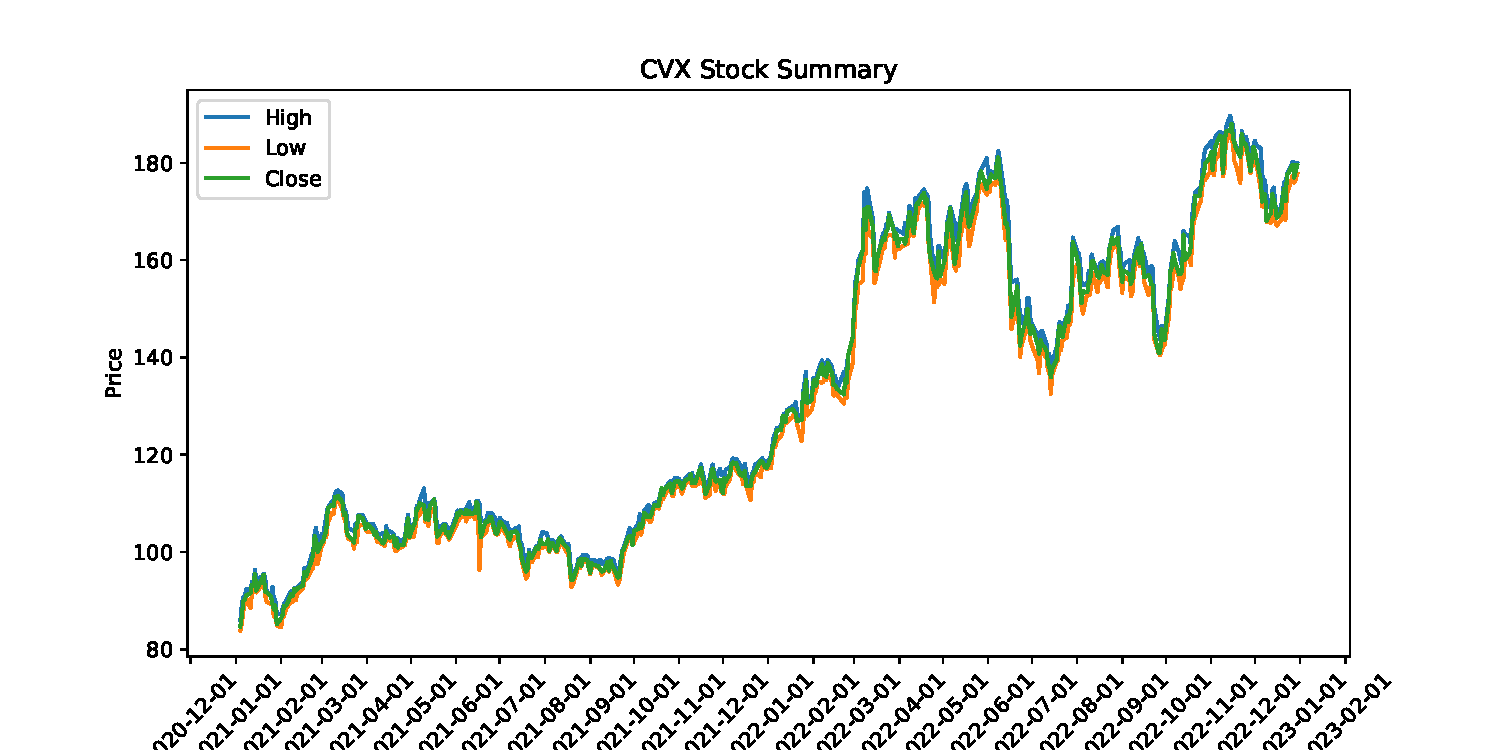
\includegraphics[width=\textwidth]{../figures/fig1.pdf}
  \caption{A plot of historic CVX stock data from 2021 to 2022}\label{fig:fig1}
  \end{center}
\end{figure}


While the Highs and Lows might be informative in analysis, in order to concentrate the focus of this paper in a manner more similar to other financial data analyses, we will only experiment the Closing Price and the Returns which can be taken by taking the log difference of the Closing Prices.	

\jy{The upper panel is repeating. Only keep one.}
\begin{figure}[!hb]
  \begin{center}
  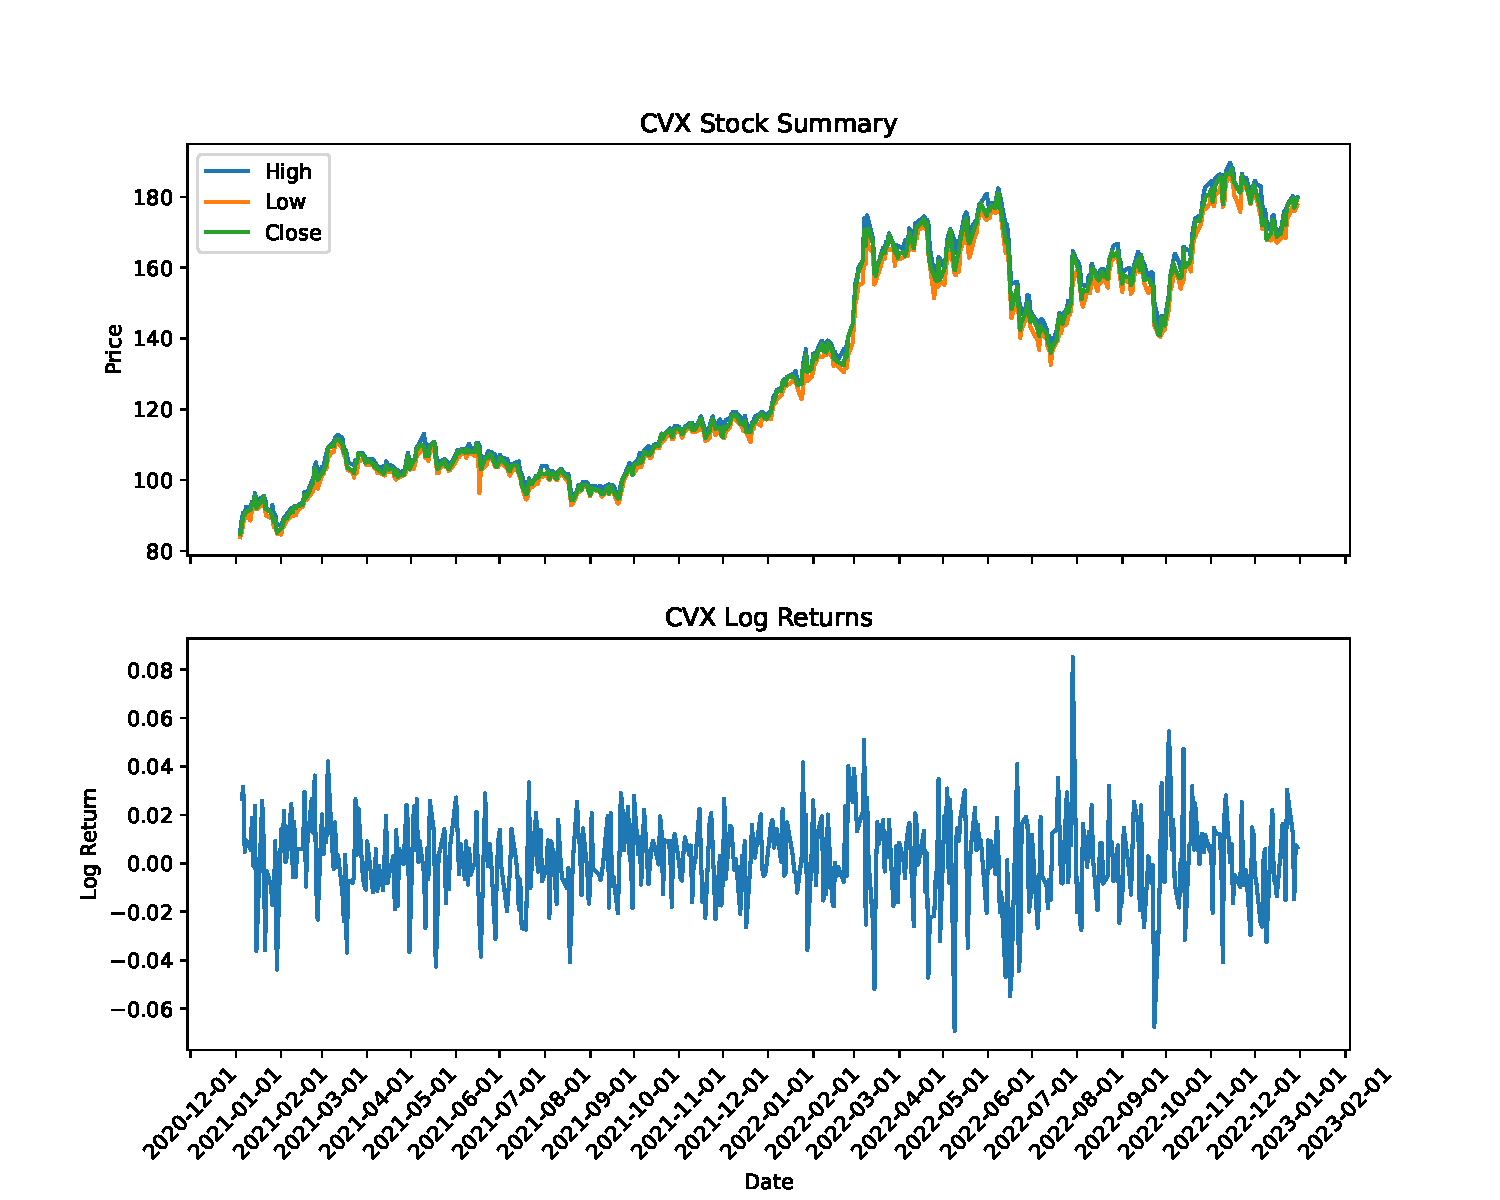
\includegraphics[width=\textwidth]{../figures/fig2.pdf}
  \caption{A plot of historic CVX stock data from 2021 to 2022 and the returns}\label{fig:fig2}
  \end{center}
\end{figure}


\jy{Use table styles from my template}
We also used the data processing library Pandas in order to generate summary statistics as shown below:
\begin{table}[!hb]
  \begin{center}
    \caption{Summary Statistics for the Chevron Stock data}
    \label{tab:table1}
    \begin{tabular}{l|c|r} % <-- Alignments: 1st column left, 2nd middle and 3rd right, with vertical lines in between
      \textbf{Metrics} & \textbf{Close} & \textbf{Returns}\\
      \hline
      count & 503.000000 & 502.000000\\
      mean & 131.520815 & 0.001496\\
      std & 30.228298 & 0.018412\\
      min & 84.709999	 & - 0.069374\\
      25\% & 103.989998 & -0.008429\\
      50\% & 118.790001 & 0.002891\\
      75\% & 160.619995 & 0.013058\\
      max & 188.050003 & 0.085292\\
    \end{tabular}
  \end{center}
\end{table}



The range of the closing values for the observed period was 84.70 to 188.05; the lowest and highest values were observed on January 4th, 2021 November 15th, 2022. There are 502 days that the stock data was available for since Chevron is a part of the New York Stock Exchange which is closed all day on Saturdays, Sundays and nine holidays a year. This was something that was taken into consideration when working with twitter data. 


The twitter data was scraped using the python package snscrape \citep{justanotherarchivist_2022}. This is an open source library that allows for the scraping of twitter data without having to use the API. The code used to generate the twitter data can be found in code/datagen.py. In short, the process used to scrape the data was to first create some auxiliary functions for tasks such as determining how many tweets need to be gathered at a given time and create some functions to make it easier to pass in queries in the Twitter Search Scraper object. Regarding the collection of tweets, the query can either be for some topic keywords or the tweets from a specific user. 


For the purpose of this paper, 10 tweets were scraped with the topic query "CVX" from January 1st 2021 to December 31st 2022.  7290 tweets were generated, saved as a csv and merged with the CVX stock data on the Date axis after matching datatypes. This also omitted tweets which were created when the stock market was closed in order to simplify the analysis. Using this we were able to perform sentiment analysis and calculate correlation.


%%%%%%%%%%%%%%%%%%%%%%%%%%%%%%%%%%%%%%%%%%%%%%%
\label{sec: methods}
\section{Methods}

\subsection{Sentiment Analysis}
\paragraph{The Transformer Model}
As mentioned in the first section, Transformers models have shown a lot of promise for a variety of natural language processing tasks, outperforming its competitors in speed and accuracy. The BERT model seems to be particularly well suited for tasks of sentiment analysis. Transformers work based on the concept of "attention" which was introduced in "Attention is all you need" \citep{vaswani2017attention} . Attention allows Transformers to learn the relationships between the words in a sentence or sequence of words. To do this, the Transformer splits the input sequence into tokens (usually individual words or sub-words) and embeds them into a high-dimensional vector space. It then applies multiple layers of self-attention, where each token in the sequence is given a weight based on its relevance to the other tokens. The self-attention mechanism allows the model to focus on the most important parts of the input sequence and learn dependencies between the words. After the self-attention layers, the Transformer applies feedforward neural networks to further refine the representations of the tokens. Transformers create differential weights signaling which words in a sentence are the most critical to further process. 	

\begin{figure}[tbp]
\tikzset{every picture/.style={line width=0.75pt}} %set default line width to 0.75pt        
\begin{tikzpicture}[x=0.75pt,y=0.75pt,yscale=-1,xscale=1]
%uncomment if require: \path (0,300); %set diagram left start at 0, and has height of 300
%Rounded Rect [id:dp4434986972980839] 
\draw   (100,43.8) .. controls (100,32.76) and (108.95,23.8) .. (120,23.8) -- (261,23.8) .. controls (272.05,23.8) and (281,32.76) .. (281,43.8) -- (281,103.8) .. controls (281,114.85) and (272.05,123.8) .. (261,123.8) -- (120,123.8) .. controls (108.95,123.8) and (100,114.85) .. (100,103.8) -- cycle ;
%Rounded Rect [id:dp8739677930569794] 
\draw   (359,68.2) .. controls (359,52.52) and (371.72,39.8) .. (387.4,39.8) -- (472.6,39.8) .. controls (488.28,39.8) and (501,52.52) .. (501,68.2) -- (501,168.4) .. controls (501,184.09) and (488.28,196.8) .. (472.6,196.8) -- (387.4,196.8) .. controls (371.72,196.8) and (359,184.09) .. (359,168.4) -- cycle ;
%Curve Lines [id:da9359490056283244] 
\draw    (282,73) .. controls (362,56.8) and (275,143.8) .. (359,124.8) ;
%Straight Lines [id:da03881732608220867] 
\draw    (78,72.8) -- (101,73) ;
%Straight Lines [id:da6091063106538472] 
\draw    (500,120.8) -- (523,121) ;
%Straight Lines [id:da19347919375178857] 
\draw    (431,215.8) -- (431,199.8) ;
% Text Node
\draw (161,65) node [anchor=north west][inner sep=0.75pt]   [align=left] {Encoder};
% Text Node
\draw (398,103) node [anchor=north west][inner sep=0.75pt]   [align=left] {Decoder};
% Text Node
\draw (42,63) node [anchor=north west][inner sep=0.75pt]   [align=left] {Input};
% Text Node
\draw (524,112) node [anchor=north west][inner sep=0.75pt]   [align=left] {Output};
% Text Node
\draw (408,219) node [anchor=north west][inner sep=0.75pt]   [align=left] { Output Probabilites};
\end{tikzpicture}
\caption{In this figure we can observe a very simplified version of the Transformer model with its two major components, the encoder and the decoder \citep{devlin2018bert}.}
\label{fig:fig2}
\end{figure}
The Transformer architecture consists of two main components: an encoder and a decoder.The encoder takes in the input sequence and generates a sequence of hidden representations, which are then passed to the decoder. The decoder then uses the encoder's output to generate the final output sequence.


We will be utilizing Bidirectional Encoder Representations from Transformers (BERT) for our sentiment analysis. BERT is a transformer model developed by Google that can perform multiple Natural Language Processing tasks such as sentiment analysis, text classification, chatbots, text extraction, machine translation, text summarization, market intelligence, auto-correct, intent classification, urgency detection, and speech recognition.


This model was initially trained on Wikipedia and Google’s BooksCorpus which contain 2,500,000,000 words and 800,000,000 words respectively. Training of BERT was completed over a period of 4 days using 64 Tensor Processing Units running in parallel. With this much data, it is able to understand context clues making it a very effective model for the purposes of sentiment analysis.


We will be specifically using distil-BERT which is a version of BERT with 12 transformation layers, and 768 Hidden Layers.\citep{muller_2022} This is more reasonable for the task we have at hand and we will implement this using the Hugging Face transformers pipeline package\citep{huggingface2023}. For each day, the average sentiment score of all tweets was calculated. Sentiment scores range from -1 to 1, where -1 represents a very negative sentiment and 1 represents a very positive sentiment.

\subsection{ARMA-GARCH Modeling}
The daily returns for Chevron's stock (CVX) were obtained from calculating as the daily logarithmic difference of the closing prices. ARMA-GARCH modeling was then performed to investigate the relationship between the daily returns and the sentiment scores.

First, an ARMA model was selected for the returns using the \texttt{auto.arima} function in the forecast package in R. The \texttt{max.D} and \texttt{max.d} parameters were set to 0 to avoid differencing in the ARMA model.

Next, a GARCH model was fitted to the ARMA residuals using the \texttt{ugarchfit} function in the rugarch package in R. The sGARCH model was used for the variance with an order of (1,1) and the mean was modeled using the ARMA model selected earlier.

To investigate the impact of sentiment on stock returns, an ARIMAX model was fitted to the returns using the \texttt{arimax} function in the TSA package in R. The daily sentiment scores were included as an exogenous variable. An ARIMAX model was also fitted to the sentiment scores using the \texttt{auto.arima} function in the forecast package in R.

Finally, a GARCHX model was fitted to the returns with sentiment scores using the \texttt{garchx} function in the garchx package in R. The order was set to (1,1), and the initial values for the GARCH coefficients were taken from the ARMA-GARCH model.

For further analysis, a weighted sentiment score was calculated by assigning a weight to each sentiment score based on the number of tweets collected for that day. The weighted sentiment score was then used as an exogenous variable in the ARIMAX and GARCHX models, and the results were compared to those obtained using the unweighted sentiment score.

%%%%%%%%%%%%%%%%%%%%%%%%%%%%%%%%%%%%%%%%%%%%%%%
\label{sec: results}
\section{Results}

The sentiment analysis took approximately 12 minutes to run and the data generated created 3 new columns in the working dataframe: sentiment, label, and score. Score is a numeric value from the range [0,1] where the higher the score the more confident the sentiment analyzed is correct. This score is the confidence that the model gives for the sentiment assignment and serves as a way to observe sentiment as a continuous variable. When combined and observed as a frequency histogram, it seems that the sentiment scores for the period are centered around a slightly positive value of 0.1 indicating sentiment for the CVX term was generally positive but normally distributed more or less.


\begin{figure}[tbp]
  \begin{center}
  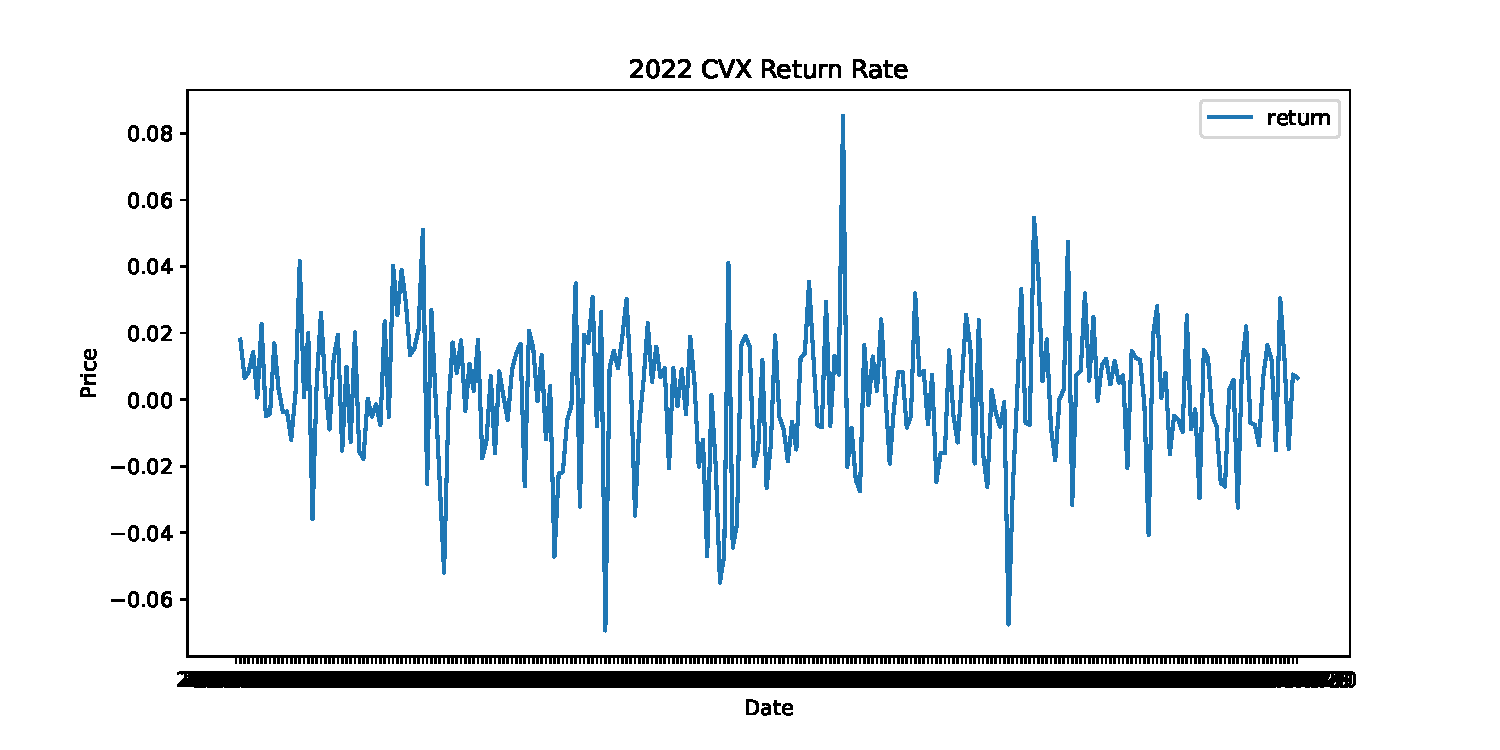
\includegraphics[width=\textwidth]{../figures/fig3.pdf}
  \caption{Sentiment Distribution }\label{fig:fig2}
  \end{center}
\end{figure}



ARMA-GARCH models have several assumptions, including the stationarity of the time series data, the presence of autoregressive and moving average processes, the normality and lack of autocorrelation in the residuals, the constant conditional variance of the data, the absence of autoregressive conditional heteroscedasticity effects, and a sufficient sample size. These assumptions are important to ensure unbiased parameter estimates and accurate predictions. Some of these assumptions such as the normality and lack of autocorrelation in the residuals, the constant conditional variance of the data, the absence of autoregressive conditional heteroscedasticity effects were checked manually by making plots using R as such:

\jy{reference to figures/tables by their labels. Never H or h. Always tbp for floating locations.}
\begin{figure}[!hb]
  \begin{center}
  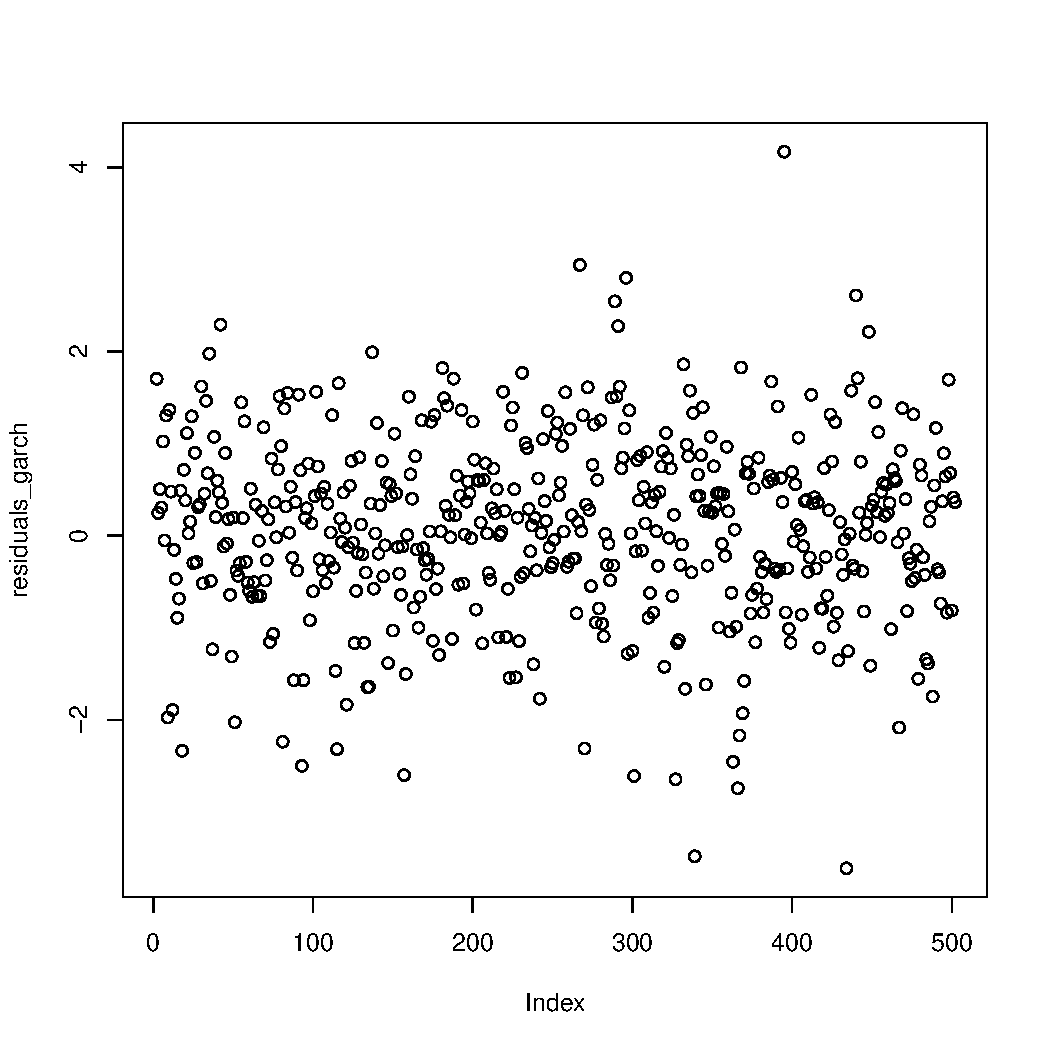
\includegraphics[width=\textwidth]{../figures/fig4.pdf}
  \caption{Garch Model Residuals}\label{fig:fig1}
  \end{center}
\end{figure}

\jy{a blank line means a new paragraph}

and those that remained were checked by the rugarch\citep{rugarch}, readr\citep{readr}, forecast\citep{forecast}, tseries\citep{tseries}, garchx\citep{garchx}, and TSA\citep{TSA} packages.
\jy{space before citep}


In the analysis, an ARMA-GARCH model was first created only using the daily sentiment and then comparing to an ARMA-GARCH model with daily sentiment as an exogenous variable. The ARMA part of this technique, models the autocorrelation and moving average patterns in the data and GARCH models the volatility or conditional heteroskedasticity of the data. To determine whether daily sentiment, the exogenous variable has any effect on the model, we conducted the Likelihood ratio test. The log likelihood values for the base model and the model with sentiment as a variable are 1293.56 and 504.85, respectively.

A higher log likelihood value indicates a better fit to the data. Therefore, based on the log likelihood values, the ARIMA(0,0,0) model with non-zero mean fits the returns better than the one which includes the sentiment score as an exogenous variable therefore, we could not reject the null hypothesis that the exogenous variable has no effect on the model. We tried this same technique by applying a weight to the sentiment score and obtained similar results.

%%%%%%%%%%%%%%%%%%%%%%%%%%%%%%%%%%%%%%%%%%%%%%%
\label{sec: discussion}
\section{Discussion}

As mentioned before, this paper is the first one to take the approach of using Transformers to determine whether twitter sentiment is informative in predicting the volatility of the stock price of the Chevron Corporation. In summary, this paper accomplished this task through the following:
\begin{itemize}
    \item Introducing some background behind the Chevron Corporation and Sentiment Analysis as a Practice.
    \item Describing the data and the methods by which the data was obtained.
    \item Describing the methods behind the sentiment analysis and correlation derivation.
    \item Describing the results.
\end{itemize}

\jy{close figure/table captions with a period.}



\jy{no need for paragraph titles}
\paragraph{Possible Expansions}
One possible expansion of this study would be to increase the sample size to include more observations and thus increase the robustness of the analysis. This would allow for more accurate statistical tests and a better understanding of the relationship between sentiment and stock price movement/volatility. Another possible expansion would be to test for causality using techniques like the Granger causality test, which would allow us to determine whether sentiment scores are truly predictive of stock price movements or whether they are just correlated. Additionally, conducting a meta-analysis of multiple companies in the fossil fuel industry or across multiple industries could provide broader insights into the relationship between sentiment and stock prices. 


\paragraph{Takeaways}
Although this study found that both weighted and unweighted sentiment scores may not have been effective in predicting stock price movement and volatility of CVX, it established a novel methodology for analyzing Twitter sentiment data and determining whether it is informative in predicting stock prices. This methodology can be applied to other industries and sectors to gain a better understanding of the role that sentiment plays in stock price movements. The methodology can be useful for multiple groups, such as Public Relations departments in companies like Chevron, who can use this to assess the effectiveness of their publicity campaigns on the company's valuation, leading to higher profits and public influence. Alternatively, environmental groups can use this methodology to measure the effectiveness of their activism campaigns in influencing the trading power of Chevron Stock ownership. This methodology provides a way for various groups to adjust their strategies to influence public sentiment and in turn stock value.

\paragraph{Conclusion}
Overall, this study provides valuable insights into the use of Twitter sentiment analysis as a tool for predicting stock prices, and points towards potential avenues for further research. With further research, determined but analyzing the effect of public sentiment on stock prices of fossil fuel companies can provide valuable insight into how public opinion can be used to augment or reduce the effects of climate change.

\jy{no manually controlled spacing}

\bibliographystyle{chicago}
\bibliography{references}

\end{document}
